

% Nastaven� �ablony FM TUL
% nastaveni prezentace
%\documentclass[draft]{beamer}
\documentclass[t]{beamer}

\usepackage[czech]{babel}

% FONTY

%\usepackage[cp1250]{inputenc} % pro win1250
\usepackage[T1]{fontenc}

\usepackage[utf8]{inputenc}
%\usepackage[IL2]{fontenc}

\usepackage{lmodern}

% XeLaTeX
%\usepackage{fontspec,lipsum}
%\defaultfontfeatures{Ligatures=TeX}
%\usepackage[small,sf,bf]{titlesec}
% 
%\setromanfont{Georgia}
%\setsansfont{Myriad Pro} %Tahoma}
%\setsansfont{Tahoma}
%\setsansfont{Arial}
%\setsansfont{Times New Roman}
%====

% bohu�el dal�� fonty nejsou pln� po�e�t�n�, tedy nejde bez obt��� kop�rovat z PDF

%\usepackage{times}
% \usepackage{avant}
% \usepackage{bookman}
% \usepackage{helvet}  %chyb� tu�n� �ez u strojov�ho p�sma
% \usepackage{newcent}
% \usepackage{palatino} 



%\usepackage[scaled]{uarial}
%\usepackage{helvet}


\usepackage{hyperref}

\mode<presentation>
{
  \definecolor{FM_TUL}{cmyk}{0,0.6,1,0}
  
  \useinnertheme{rectangles}
  
  % VN�J�� BAREVN� T�MA NADPIS�    
  \usecolortheme{whale}  
  
  % VNIT�N� BAREVN� T�MA V��T�, BLOK� ATD.  
  \usecolortheme{orchid}

  \setbeamercolor{titlelike}{parent=structure}
  \setbeamercolor{frametitle}{fg=black}
  \setbeamercolor{title}{fg=black}
  \setbeamercolor{item}{fg=FM_TUL} 
  \setbeamertemplate{navigation symbols}{} % potla�en� naviga�n�ch symbol�
  \setbeamercolor{block title}{fg=white,bg=FM_TUL} % p�edefinov�n� barvy z�kl. bloku
  \setbeamercolor{caption name}{fg=FM_TUL}
  
%  Nadpisy slid� tu�n� dokud nevy�e��m pou�it� font� tak, aby se dalo kop�rovat z pdf
%  \setbeamercolor{frametitle}{fg=FM_TUL}
  \setbeamertemplate{frametitle}
  {
    \textbf{\insertframetitle}
    \par
  }
  \setbeamercolor{bibliography entry author}{fg=black} % literatura �ern� a ne mod�e
  \setbeamercolor{bibliography entry title}{fg=black} % literatura �ern� a ne mod�e
  \setbeamercolor{bibliography entry journal}{fg=black} % literatura �ern� a ne mod�e
  \setbeamercolor{bibliography entry note}{fg=black} % literatura �ern� a ne mod�e
  
%Nefunguje  \setbeamercolor{tableofcontents}{fg=TUL_FM} % obsah TUL_FM a ne mod�e
}

%===============================================================================
% TITULN� STRANA
%===============================================================================
\setbeamertemplate{title page}{
\begin{flushleft}
   
\includegraphics[width=0.6\textwidth]{obr/logo-fm-cmyk-cz.pdf}
\end{flushleft} 
  %
\begin{center} 
  \setbeamercolor{postit}{fg=black,bg=FM_TUL}
%  \begin{beamercolorbox}[center,sep=2pt,wd=\textwidth,ht=3cm,dp=20pt]{postit}
 \begin{beamercolorbox}[center,sep=10pt,wd=\textwidth,ht=3.2cm,ignorebg]{postit}
            
      {\bf {\LARGE \inserttitle}}\\[16pt]
              
      \insertsubtitle
  \end{beamercolorbox}
%
  \vspace{10pt}
  {\bf \small \insertauthor {\color{FM_TUL} ~|} \insertdate}
%  \vspace{10pt}    
\end{center}
%
\vfill
\vskip0pt plus 1filll
{\color{FM_TUL} \hrule} 
%
\begin{center}
\vspace{-8pt}         
\TextTitulniStranaPodLinkou
\end{center}   
}
%===============================================================================
% Z�HLAV� KA�D�HO SLAJDU
%===============================================================================
\setbeamertemplate{headline}{
  \hspace{-3pt}
\includegraphics[width=0.3\textwidth]{obr/logo-fm-cmyk-cz.pdf}
}
%===============================================================================
\setbeamertemplate{footline}{

\includegraphics[width=\textwidth]{obr/FM_TUL_linka_piktogram_obd.pdf}

\vspace{-9.5pt}
~\hfill {\tiny\color{white} \insertframenumber\,/\,\inserttotalframenumber}\hspace{5pt}

\hspace{3pt} {\tiny \inserttitle {\color{FM_TUL} ~|} \insertdate }\hspace{3pt}
\vspace{3pt}
}
%===============================================================================
% �PRAVA BARVY TEXTU V OBSAHU 
%===============================================================================
\setbeamercolor{section in toc}{fg=black}
\setbeamercolor{subsection in toc}{fg=black}
\setbeamercolor{subsubsection in toc}{fg=black}
\setbeamercolor{button}{bg=FM_TUL}

%\definecolor{links}{HTML}{2A1B81}
\hypersetup{colorlinks,linkcolor=,urlcolor=FM_TUL}


\usepackage{palatino}
\usepackage{graphicx}
\usepackage{transparent}

\setbeamercovered{transparent=35}

\title[Pokročilý třídní jazykový slovníček]{Pokročilý třídní jazykový slovníček}
\subtitle{Diplomová práce}
\author[Bc.~Daniel~Maděra]{Bc.~Daniel~Maděra}
\institute[TUL]{Technická univerzita v Liberci}
\date{1.~února~2017}
\newcommand{\TextTitulniStranaPodLinkou}{\tiny
Studentská 2 {\color{FM_TUL} |} 461\,17 Liberec 2 {\color{FM_TUL} |} {daniel.madera@tul.cz} {\color{FM_TUL} |} 
\href{http://www.fm.tul.cz/}{www.fm.tul.cz}}

\renewcommand{\inserttotalframenumber}{\pageref{lastslide}}

\begin{document}
%\setbeamertemplate{caption}{\insertcaption}


\begin{frame}
    \titlepage
\end{frame}

\begin{frame}
    \frametitle{Obsah}
    \begin{itemize}
        \item problematika
            % - učení slovíček při hodinách -> vlastní seznamy slovíček
            % - ostatní řešení žákům neposkytují přizpůsobení úrovně ani obsahu
            % - cílem diplomové práce je provést analýzu, jak zefektivnit učení a motivovat žáky k procvičování slovíček 
            % - na základě zjištěných poznatků navrhnout a implementovat aplikaci, která umožní rozvíjet cizojazyčnou slovní zásobu % - a zároveň vyučujícím poskytne nástroj pro správu a prezentaci slovíček pro žáky
        \item představení aplikace
            % - koncept (funkcionalita)
            %     + každý může tvořit
            % - nástroj pro vyučující 
            %     + tvorba učebnic (správa slovíček, modulů)
            %         - import slov
            %         - sdílení učebnic
            %     + tvorba tříd (oddělené skupiny)
            % - nástroj pro studenty
            %     + procvičování slovíček z učebnic i vlastních
            %     + připomínání slovíček v narůstajících intervalech
            %         - permanentní zapamatování
            % - automatizované poskytnutí zvukové, obrazové a textové formy
            % - snaha o motivaci
            % zvuková forma - syntéza pomocí Google Text To Speeach API
        \item algoritmizace
            % - metoda rozloženého opakování
            %     - supermemo
            %     - adaptovaný leiterův algoritmus (obrázek)
            %         - 2 fáze (zjištění úrovně žáka, samotné procvičování)
            % - aktivní vzpomínání a rozpoznání slova
            %     - algoritmus
        % \item technologie
        \item grafické rozhraní
        \item shrnutí
    \end{itemize}
\end{frame}


\begin{frame}[t]
    \frametitle{Problematika}
    \begin{block}{Učení slovníček cizího jazyka}
    \begin{itemize}[<+->]
        \item systém vlastního slovníčku
        % neorganizované, 
        % Žáci si při výuce cizího jazyka obvykle vedou vlastní slovníček, do kterého si zapisují nově nabytá slova. V době přípravy na test rychle slova zopakují a následně z krátkodobé paměti test napíšou, což má za následek, že pokud naučená slova dále neopakují, dojde k jejich zapomenutí. Navíc se postupně slovíčka hromadí a není v silách žáka je opakovat.
        \item výukové aplikace
    \end{itemize}
    \end{block}
    
    \begin{block}{Výukové nástroje a aplikace}
    \begin{itemize}[<+->]
        \item neumožňují definici vlastních slov
        \item přizpůsobit zásobu aktuálně probírané
        \item přizpůsobení úrovni žáka
    \end{itemize}
    \end{block}
\end{frame}

\begin{frame}[c]
    \frametitle{Cíle práce}
    \begin{itemize}[<+->]
        \item vytvořit výukový nástroj
    \end{itemize}
    
    \begin{block}{Pro vyučující}
    \begin{itemize}[<+->]
        \item správa učebnic se slovíčky
        \item zpřístupnění slovíček žákům
    \end{itemize}
    \end{block}

    \begin{block}{Pro žáky}
        \begin{itemize}[<+->]
            \item naučit a procvičovat slova
            \item připomínat naučená slova
            \item zvuková, textová a obrazová forma
            \item motivovat
        \end{itemize}
    \end{block}
\end{frame}

\begin{frame}[t]
    \frametitle{Hlavní myšlenky aplikace}
    % možná obrázek místo textu
    \begin{itemize}[<+->]
        \item nejen pro vyučující a žáky (kdokoliv)
        \item sloužit jako portál
        \item sdílení učebnic
        \item tvorba testovacích sad
        \item účelem není testovat žáky
        % nemá za úkol zkoušet slovíčka, spíše usnadnit přípravu žáků na následující hodinu a zároveň rozvíjet slovní zásobu
        \item efektivně rozvíjet slovní zásobu podle probírané učebnice
        % rozvíjet slovní zásobu
        \item $\rightarrow$ algoritmy na metodě rozloženého opakování
    \end{itemize}
\end{frame}

\begin{frame}[t]
    \frametitle{Generování slov v procvičování - inicializace}
    \only<1> {\begin{center}\includegraphics[width=8cm]{./img/words-gen-algorithm.png}\end{center}}
    \only<2> {\begin{center}\includegraphics[width=8cm]{./img/words-gen-algorithm-0.png}\end{center}}
    \only<3> {\begin{center}\includegraphics[width=8cm]{./img/words-gen-algorithm-1.png}\end{center}}
    \only<4> {\begin{center}\includegraphics[width=8cm]{./img/words-gen-algorithm-2.png}\end{center}}
    \only<5> {\begin{center}\includegraphics[width=8cm]{./img/words-gen-algorithm-3.png}\end{center}}
    \only<6> {\begin{center}\includegraphics[width=8cm]{./img/words-gen-algorithm-4.png}\end{center}}
    \only<7> {\begin{center}\includegraphics[width=8cm]{./img/words-gen-algorithm-5.png}\end{center}}
    \only<8> {\begin{center}\includegraphics[width=8cm]{./img/words-gen-algorithm-6.png}\end{center}}
\end{frame}

\begin{frame}[fragile]
    \frametitle{Generování slov v procvičování - testování}
    \begin{columns}[T] % align columns
        \begin{column}{.48\textwidth}
            \only<1> {\begin{center}\includegraphics[width=\textwidth]{./img/words-gen-algorithm-leitner.png}\end{center}}
            \only<2> {\begin{center}\includegraphics[width=\textwidth]{./img/words-gen-algorithm-leitner-1.png}\end{center}}
            \only<3> {\begin{center}\includegraphics[width=\textwidth]{./img/words-gen-algorithm-leitner-2.png}\end{center}}
            \only<4> {\begin{center}\includegraphics[width=\textwidth]{./img/words-gen-algorithm-leitner-3.png}\end{center}}
            \only<5> {\begin{center}\includegraphics[width=\textwidth]{./img/words-gen-algorithm-leitner-4.png}\end{center}}
            \only<6-> {\begin{center}\includegraphics[width=\textwidth]{./img/words-gen-algorithm-leitner-5.png}\end{center}}
        \end{column}%
        \hfill%
        \begin{column}{.48\textwidth}
            \begin{block}{Testování}
                \begin{itemize}
                    \item<2-> 1. průchod
                    \item<3-> 2. průchod
                    \item<4-> 3. průchod
                    \item<5-> správná a neúplná odpověď
                    \item<6-> špatná odpověď
                    \item<7-> konec: všechna slova jsou dokončená
                \end{itemize}
            \end{block}
        \end{column}%
    \end{columns}
\end{frame}

\begin{frame}[t]
    \frametitle{Připomínání slov}
    \begin{itemize}
        \item metoda rozloženého opakování (Supermemo)
        \item intervaly: 1d, 3d, 13d, 24d, 1,7m 
    \end{itemize}
    \begin{center}
        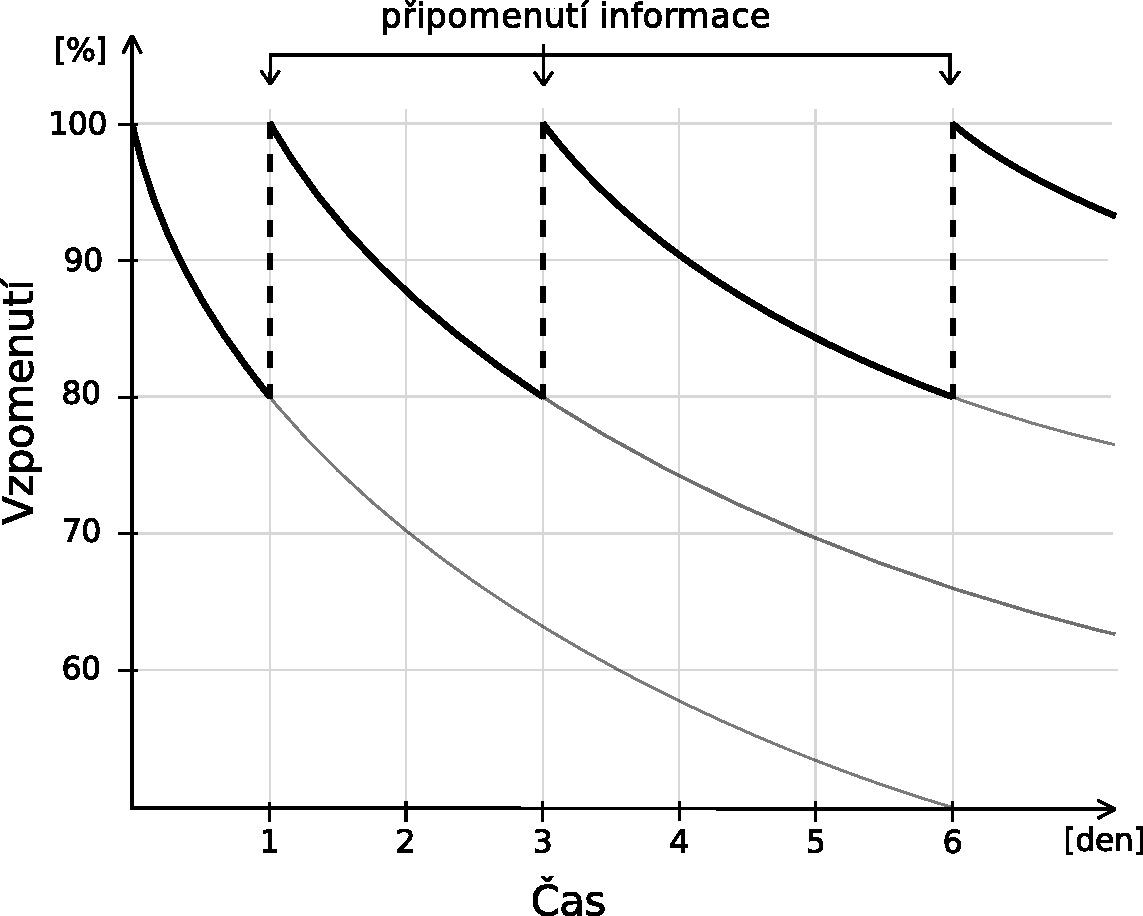
\includegraphics[width=6.5cm]{./img/forgetting-curve.pdf}\\
    \end{center}
\end{frame}

\begin{frame}[t]
    \frametitle{Grafické rozhraní}
    \begin{itemize}
        \item frontend: javscriptová SPA
        \item backend: HTTP API v Pythonu
    \end{itemize}
    \begin{center}
        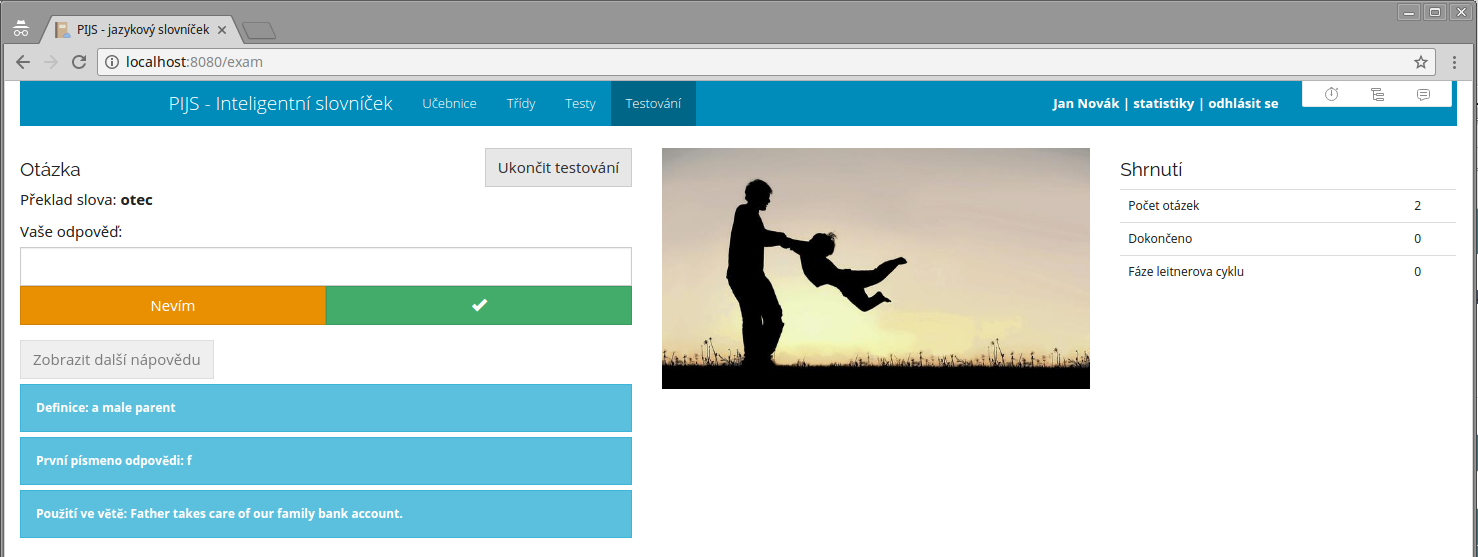
\includegraphics[width=\textwidth]{./img/gui.png}\\
    \end{center}
\end{frame}

\begin{frame}[t]
    \frametitle{Závěr}
    \begin{itemize}
        \item byla provedena rešerše existujících aplikací 
        \item byla navržena a implentována aplikace
        \item umožňuje správu slovíček, tříd a testovacích sad
        \item umožňuje automaticky získat další interpretační formy slova (zvuk, obrázek)
        \item motivující a adaptivní procvičování
        \item připomínání slovíček v efektivních intervalech
        \item testování aplikace externími uživateli
    \end{itemize}
\end{frame}


\begin{frame}
\begin{center}
\label{lastslide}
\huge Děkuji za pozornost.
\end{center}
\end{frame}

\begin{frame}[noframenumbering]
\begin{center}
    \frametitle{Existují další možnosti stanovení obtížnosti slovíček? Jakým způsobem by změna metody ovlivnila aplikaci?}
    % ohledně globální obtížnosti...
    % - aktuálně globání obtížnost je tvořena váženým průměrem v podobě délky slov, podobnost s výrazem v mateřekém jazyce a výskyt speciálních znaků jako přehlasovaná písmena, dvojitý výskyt apod.
    % mohlo by se zakomponovat do průměru i hodnota, jak často se na slovo v daném jazyku naráží - most frequent words
    % ještě lepší vyhodnocení obtížnosti na základě fonetické podobnosti - aktuálně se porovnává Levenshteinovou vzdáleností
    % vyhodnocovat obtížnost slova statisticky -> problém, ale že na začátku jsou data prázdná

    % aplikaci by změna metody neovlivnila, bylo by nutné návratovou hodnotu nové metody normalizovat do intervalu <0,1)

\end{center}
\end{frame}

\begin{frame}[noframenumbering]
\begin{center}
    \frametitle{Jaký může být důsledek toho, že není použito API dle REST ale vlastní řešení?}
    % api nemusí být intuitivní, což může ztěžovat případné rozšíření dalších klientů používajícíh APi.
    % například při programování nového klienta komunikující s API se bude muset nastudovat struktura, jelikož aktuální API nevyužívá princip RESTful, kde společně s daty se zasílá i hypertextové odkazy představující další stavy aplikace
    % myšlenka stejně byla hodně logiky (generování slovíček apod.) přesunout na klienta, API slouží pouze jako úložiště 
\end{center}
\end{frame}

\begin{frame}[noframenumbering]
\begin{center}
    \frametitle{Pro práci byla zvolena integrace se službami Google. Byly zvažovány i další možnosti, např. integrace výkladového slovníku apod.?}
    % pouze k doplnění ke slovu je možné uložit i definici a použití ve větě
    % ano byla zvážena možnost výkladového slovníku, ale nakonec se od této možnosti distancovalo, jelikož každý vyučující může slovo definovat žákům v hodinách po svém a mohlo by dojít k žáci by potom cizím definicím nemuseli porozumět
    % zároveň vyučující přizpůsobí definici slov dle vlastního uvážení - bude využívat takovou slovní zásobu, která odpovídá úrovni žáků
    % další možností, která byla v úvaze, bylo získávat překlad slova, ale znovu by vyučující mohli narážet na problém, že významy slov zcela nekorespondují s těmi, které sdělovali dětem - například více významová slova

\end{center}
\end{frame}

\end{document}
